\documentclass[10pt,a4paper]{article}
\usepackage[margin=2cm]{geometry}
\usepackage{amsmath,amssymb}
\usepackage{booktabs}
\usepackage{graphicx}
\usepackage{float}
\usepackage[hidelinks]{hyperref}
\usepackage{caption}
\captionsetup{font=small}

\title{Equilibrium solvers for the Competition for Risk game:\\ approaches and benchmark}
\author{Louis Abraham}
\date{September 2026}

\begin{document}
\maketitle

\begin{abstract}
We compare our regret-matching solvers with 21 other methods that compute Nash equilibria of the
two-player Competition for Risk (CfR) game with market friction $\tau$ and correlated failures
$\rho$ \cite{abraham2023}. All methods are evaluated with the same metric, the QuasiNashConv with
continuous best responses, and the same time limit. We then add a new method, Double Oracle
followed by a Newton solve on the atom positions, and we solve the $n$-player game with friction
with the Multiple Oracle algorithm \cite{kroupa2021}. The best method depends on $\tau$: support
generation for $\tau=0.03$, fictitious play for $\tau=10^{-4}$ and Newton on the complementarity
problem for $\tau=0$.
\end{abstract}

\section{Game and protocol}

\paragraph{Game.} Player $i$ picks a risk $r_i\in[0,1]$ and fails with probability $r_i$; the two
failures are correlated through a Gaussian copula with correlation $\rho$, and $\tilde r$ is the
probability that both fail. With reward $R=1$ and penalty $P$, the payoff of player 1 is
\[
u_1(r_1,r_2) = (r_2-\tilde r) - r_1 P + (1-r_1-r_2+\tilde r)\,\sigma_\tau(r_1-r_2),
\]
where $\sigma_\tau(x)=1/(1+e^{-x/\tau})$ and $\sigma_0$ is the step function (value $1/2$ on
ties). All two-player experiments use $P=1$, $\rho=0.5$ and $\tau\in\{0.03, 10^{-4}, 0\}$. For
$\tau=0.03$ the equilibrium has 6 atoms and \texttt{analytical.py} computes it exactly; for
$\tau=0$ it is a density on $[0, 0.387]$; for $\tau=10^{-4}$ no exact solution is available.

\paragraph{Quality.} The QuasiNashConv (QNC) of a profile $(p_1,p_2)$ is
$\sum_i \big(\max_{r\in[0,1]} u_i(r, p_{-i}) - u_i(p)\big)$. The maximum over $r$ is continuous,
not over the grid of the method: a Sobol scan of $2^{14}$ points, the opponent's atoms and the
points at $\pm10^{-12}$ of them (the supremum is a one-sided limit when $\tau=0$), then Brent
refinement of the 8 best points. The exact equilibrium at $\tau=0.03$ gets QNC $1.1\cdot10^{-16}$.
At $\tau=0$, the analytical density cut into 8192 equal-mass atoms gets $1.2\cdot10^{-4}$.

\paragraph{Time.} Every solve runs in its own process with one thread (BLAS, numba, Gurobi, HiGHS,
XLA), on an Apple M4 Max on AC power, with at most 10 solves in parallel (fewer than the 12
performance cores). A solve that has not finished after 120\,s returns its best point if the
solver allows it; a hard timeout kills it at 240\,s. Time is the construction of the payoff
matrix plus the solve. Grid methods use the grid $\{0, 1/(n-1), \dots, 1\}$ for both players,
with $n=16,32,\dots,4096$. For a method, the grid sizes run in increasing order and stop at the
first failure.

\paragraph{Iterations.} An iterative method runs once per $n$ and saves its strategy after
chunks of $1,1,2,4,8,\dots$ iterations, until 120\,s. Each snapshot is one point
$(n,\text{iterations})$. For every method we keep the lower envelope over all its points: the best
QNC that is reachable within a given time. One iteration of every iterative method costs $O(n^2)$:
for the sampled methods (RM, fictitious play) one ``iteration'' is a round of $n$ updates.

\section{Methods}

\begin{table}[H]
\centering\small
\begin{tabular}{p{4.6cm}p{11.6cm}}
\toprule
Method & Description \\
\midrule
RM, CFR (ours) & Regret matching with sampled updates, and its full-information version
(CFR), average strategies \cite{hart2000,zinkevich2007,abraham2023}. Also with shifted grids: the
two players use interleaved grids, as in the paper. \\
Lemke--Howson (Gambit, numpy) & Complementary pivoting on the bimatrix game \cite{lemke1964}:
Gambit in floating point \cite{gambit}, and a numpy tableau with the lexicographic ratio test,
after \cite{mathecon}. \\
Logit QRE path (Gambit) & Path of logit quantal response equilibria as $\lambda\to\infty$
\cite{mckelvey1995,turocy2005}. \\
Mangasarian--Stone QP (Gurobi) & The quadratic program of \cite{mangasarian1964}:
$\min \alpha+\beta-p^\top(A+B)q$ s.t. $Aq\le\alpha\mathbf 1$, $B^\top p\le\beta\mathbf 1$, $p,q$
in the simplex. Its global minima (value 0) are the Nash equilibria. Nonconvex, solved globally
by Gurobi. \\
Nash-gap QP, $2n$ bilinear (Gurobi, SCIP) & The same program as \cite{mangasarian1964} with
$w=Aq$ and $s=B^\top p$ as variables: the objective $\alpha+\beta-p^\top w-q^\top s$ has $2n$
bilinear terms instead of $n^2$. \\
FB-NCP Newton & Symmetric equilibrium $x$ as a complementarity problem, $x\ge0$, $v\mathbf1-Ax\ge0$,
$x^\top(v\mathbf 1-Ax)=0$, with the Fischer--Burmeister function \cite{fischer1992}, smoothing and
damped Newton steps. \\
Ipopt multi-start & The symmetric Nash-gap program, local interior-point solves \cite{ipopt} from 5
starts. \\
Double Oracle, grid / continuous & Restricted game on a growing support; each iteration adds up to
8 profitable local maxima of the deviation payoff per player \cite{mcmahan2003}. Best responses on
the grid, or over $[0,1]$ (Sobol scan of $n$ points and Brent refinement). \\
Double Oracle + Newton & New: Section~\ref{sec:hybrid}. \\
Fictitious play, Hedge, replicator & Simultaneous fictitious play \cite{brown1951,robinson1951},
multiplicative weights with step $\eta_t=\sqrt{8\log n/t}$ \cite{freund1999}, discrete replicator
dynamics \cite{taylor1978}. \\
nashopt: MILP (HiGHS, Gurobi), Lemke, GNEP, extragradient, DR-DAQP & The bimatrix game as a
linear-quadratic generalized Nash problem in nashopt \cite{nashopt}: big-M mixed-integer program
of the KKT conditions (the approach of \cite{sandholm2005}), Lemke's algorithm, least squares on
the Fischer--Burmeister KKT residual, extragradient \cite{korpelevich1976}, Douglas--Rachford with
active set. \\
\bottomrule
\end{tabular}
\caption{The 24 methods. The solvers that need a monotone game (nashopt \texttt{qp\_gnep},
\texttt{op\_extrap}) do not apply: the pseudo-gradient of this game is not monotone.}
\end{table}

\section{Results}

Table~\ref{tab:all} gives the best QNC of each method over the whole run, and
Table~\ref{tab:10s} the best QNC within 10\,s. Figure~\ref{fig:tradeoff} shows the lower
envelopes. Full tables, with the $n$ and iteration counts of each point and the first failing
grid size of each method, are in \texttt{bench/tau=*/RESULTS.md} and \texttt{bench/SUMMARY.md}.

\begin{table}[H]
\centering\small
\begin{tabular}{lccc}
\toprule
Method & $\tau=0.03$ & $\tau=10^{-4}$ & $\tau=0$ \\
\midrule
Double Oracle + Newton on atoms & $6.7\cdot10^{-16}$ (2.8 s) & $8.2\cdot10^{-3}$ (90 s) & -- \\
Double Oracle, continuous BR & $2.9\cdot10^{-11}$ (2.5 s) & $6.7\cdot10^{-3}$ (120 s) & $8.2\cdot10^{-3}$ (31 s) \\
Double Oracle, grid BR & $9.0\cdot10^{-8}$ (2.5 s) & $5.1\cdot10^{-3}$ (15 s) & $6.8\cdot10^{-3}$ (15 s) \\
FB-NCP Newton, symmetric & $9.0\cdot10^{-8}$ (9.8 s) & $8.5\cdot10^{-5}$ (128 s) & $8.4\cdot10^{-4}$ (128 s) \\
Lemke-Howson (numpy tableau) & $9.0\cdot10^{-8}$ (34 s) & $2.1\cdot10^{-2}$ (0.44 s) & $2.3\cdot10^{-2}$ (0.44 s) \\
Fictitious play & $1.1\cdot10^{-7}$ (88 s) & $6.7\cdot10^{-5}$ (84 s) & $9.2\cdot10^{-4}$ (51 s) \\
nashopt Lemke & $1.7\cdot10^{-6}$ (46 s) & $6.8\cdot10^{-3}$ (17 s) & $8.7\cdot10^{-3}$ (13 s) \\
Nash-gap QP, 2n bilinear (Gurobi) & $3.7\cdot10^{-6}$ (121 s) & $6.9\cdot10^{-4}$ (121 s) & $2.0\cdot10^{-3}$ (121 s) \\
Ipopt multi-start & $4.7\cdot10^{-6}$ (97 s) & $7.5\cdot10^{-4}$ (44 s) & $2.0\cdot10^{-3}$ (50 s) \\
Nash-gap QP, 2n bilinear (SCIP) & $5.2\cdot10^{-6}$ (124 s) & $7.2\cdot10^{-4}$ (21 s) & $2.0\cdot10^{-3}$ (29 s) \\
Replicator dynamics & $8.8\cdot10^{-6}$ (35 s) & $2.0\cdot10^{-3}$ (93 s) & $3.4\cdot10^{-3}$ (68 s) \\
Mangasarian-Stone QP (Gurobi) & $1.0\cdot10^{-5}$ (120 s) & $6.8\cdot10^{-3}$ (120 s) & $8.7\cdot10^{-3}$ (120 s) \\
CFR (ours) & $2.2\cdot10^{-5}$ (66 s) & $2.1\cdot10^{-4}$ (120 s) & $1.3\cdot10^{-3}$ (74 s) \\
Logit QRE path (Gambit) & $3.6\cdot10^{-5}$ (74 s) & $6.8\cdot10^{-3}$ (22 s) & $8.7\cdot10^{-3}$ (24 s) \\
Multiplicative weights & $2.8\cdot10^{-4}$ (91 s) & $6.0\cdot10^{-4}$ (101 s) & $1.5\cdot10^{-3}$ (128 s) \\
nashopt extragradient & $3.1\cdot10^{-4}$ (74 s) & $1.1\cdot10^{-2}$ (68 s) & $1.3\cdot10^{-2}$ (81 s) \\
RM (ours), shifted grids & $6.2\cdot10^{-4}$ (102 s) & $7.3\cdot10^{-4}$ (103 s) & $1.6\cdot10^{-3}$ (94 s) \\
RM (ours) & $7.4\cdot10^{-4}$ (12 s) & $7.8\cdot10^{-4}$ (101 s) & $1.6\cdot10^{-3}$ (93 s) \\
nashopt MILP (Gurobi) & $7.5\cdot10^{-4}$ (13 s) & $4.2\cdot10^{-2}$ (0.87 s) & $4.4\cdot10^{-2}$ (0.73 s) \\
nashopt MILP (HiGHS) & $7.8\cdot10^{-4}$ (117 s) & $6.8\cdot10^{-3}$ (37 s) & $8.7\cdot10^{-3}$ (36 s) \\
Lemke-Howson (Gambit) & $7.8\cdot10^{-4}$ (0.057 s) & $6.8\cdot10^{-3}$ (204 s) & $8.7\cdot10^{-3}$ (198 s) \\
CFR (ours), shifted grids & $8.5\cdot10^{-4}$ (6.7 s) & $1.1\cdot10^{-3}$ (122 s) & $2.0\cdot10^{-3}$ (60 s) \\
nashopt GNEP (FB least squares) & $3.1\cdot10^{-3}$ (0.93 s) & $4.2\cdot10^{-2}$ (5.3 s) & $4.4\cdot10^{-2}$ (4.1 s) \\
nashopt DR-DAQP & $2.6\cdot10^{-2}$ (0.00088 s) & $7.2\cdot10^{-4}$ (113 s) & $2.0\cdot10^{-3}$ (96 s) \\
\bottomrule
\end{tabular}

\caption{Best QNC over the whole run (time in brackets), sorted by the result at $\tau=0.03$.
``--'': no result (failure at the smallest grids, or not applicable).}
\label{tab:all}
\end{table}

\begin{table}[H]
\centering\small
\begin{tabular}{lccc}
\toprule
Method & $\tau=0.03$ & $\tau=10^{-4}$ & $\tau=0$ \\
\midrule
Double Oracle + Newton on atoms & $6.7\cdot10^{-16}$ & -- & -- \\
Double Oracle, continuous BR & $2.9\cdot10^{-11}$ & -- & $1.1\cdot10^{-2}$ \\
Double Oracle, grid BR & $9.0\cdot10^{-8}$ & $6.8\cdot10^{-3}$ & $8.7\cdot10^{-3}$ \\
FB-NCP Newton, symmetric & $9.0\cdot10^{-8}$ & $7.2\cdot10^{-4}$ & $2.0\cdot10^{-3}$ \\
Lemke-Howson (numpy tableau) & $1.7\cdot10^{-6}$ & $2.1\cdot10^{-2}$ & $2.3\cdot10^{-2}$ \\
Fictitious play & $1.3\cdot10^{-6}$ & $5.5\cdot10^{-4}$ & $1.3\cdot10^{-3}$ \\
nashopt Lemke & $9.3\cdot10^{-6}$ & $2.1\cdot10^{-2}$ & $2.3\cdot10^{-2}$ \\
Nash-gap QP, 2n bilinear (Gurobi) & $7.8\cdot10^{-4}$ & $1.2\cdot10^{-1}$ & $1.3\cdot10^{-1}$ \\
Ipopt multi-start & $3.5\cdot10^{-5}$ & $6.8\cdot10^{-3}$ & $8.7\cdot10^{-3}$ \\
Nash-gap QP, 2n bilinear (SCIP) & $9.2\cdot10^{-6}$ & $5.1\cdot10^{-3}$ & $6.8\cdot10^{-3}$ \\
Replicator dynamics & $1.5\cdot10^{-5}$ & $6.5\cdot10^{-3}$ & $7.9\cdot10^{-3}$ \\
Mangasarian-Stone QP (Gurobi) & $7.8\cdot10^{-4}$ & $1.2\cdot10^{-1}$ & $4.4\cdot10^{-2}$ \\
CFR (ours) & $5.1\cdot10^{-5}$ & $8.6\cdot10^{-4}$ & $2.1\cdot10^{-3}$ \\
Logit QRE path (Gambit) & $1.6\cdot10^{-4}$ & $2.1\cdot10^{-2}$ & $2.3\cdot10^{-2}$ \\
Multiplicative weights & $8.0\cdot10^{-4}$ & $1.7\cdot10^{-3}$ & $3.1\cdot10^{-3}$ \\
nashopt extragradient & $9.5\cdot10^{-4}$ & $2.8\cdot10^{-2}$ & $3.1\cdot10^{-2}$ \\
RM (ours), shifted grids & $1.0\cdot10^{-3}$ & $2.0\cdot10^{-3}$ & $3.1\cdot10^{-3}$ \\
RM (ours) & $1.0\cdot10^{-3}$ & $2.1\cdot10^{-3}$ & $3.1\cdot10^{-3}$ \\
nashopt MILP (Gurobi) & $3.1\cdot10^{-3}$ & $4.2\cdot10^{-2}$ & $4.4\cdot10^{-2}$ \\
nashopt MILP (HiGHS) & $3.1\cdot10^{-3}$ & $4.2\cdot10^{-2}$ & $4.4\cdot10^{-2}$ \\
Lemke-Howson (Gambit) & $7.8\cdot10^{-4}$ & $2.1\cdot10^{-2}$ & $2.3\cdot10^{-2}$ \\
CFR (ours), shifted grids & $8.5\cdot10^{-4}$ & $1.9\cdot10^{-3}$ & $2.6\cdot10^{-3}$ \\
nashopt GNEP (FB least squares) & $3.1\cdot10^{-3}$ & $4.2\cdot10^{-2}$ & $4.4\cdot10^{-2}$ \\
nashopt DR-DAQP & $2.6\cdot10^{-2}$ & $6.8\cdot10^{-3}$ & $8.7\cdot10^{-3}$ \\
\bottomrule
\end{tabular}

\caption{Best QNC within 10\,s.}
\label{tab:10s}
\end{table}

\begin{figure}[p]
\centering
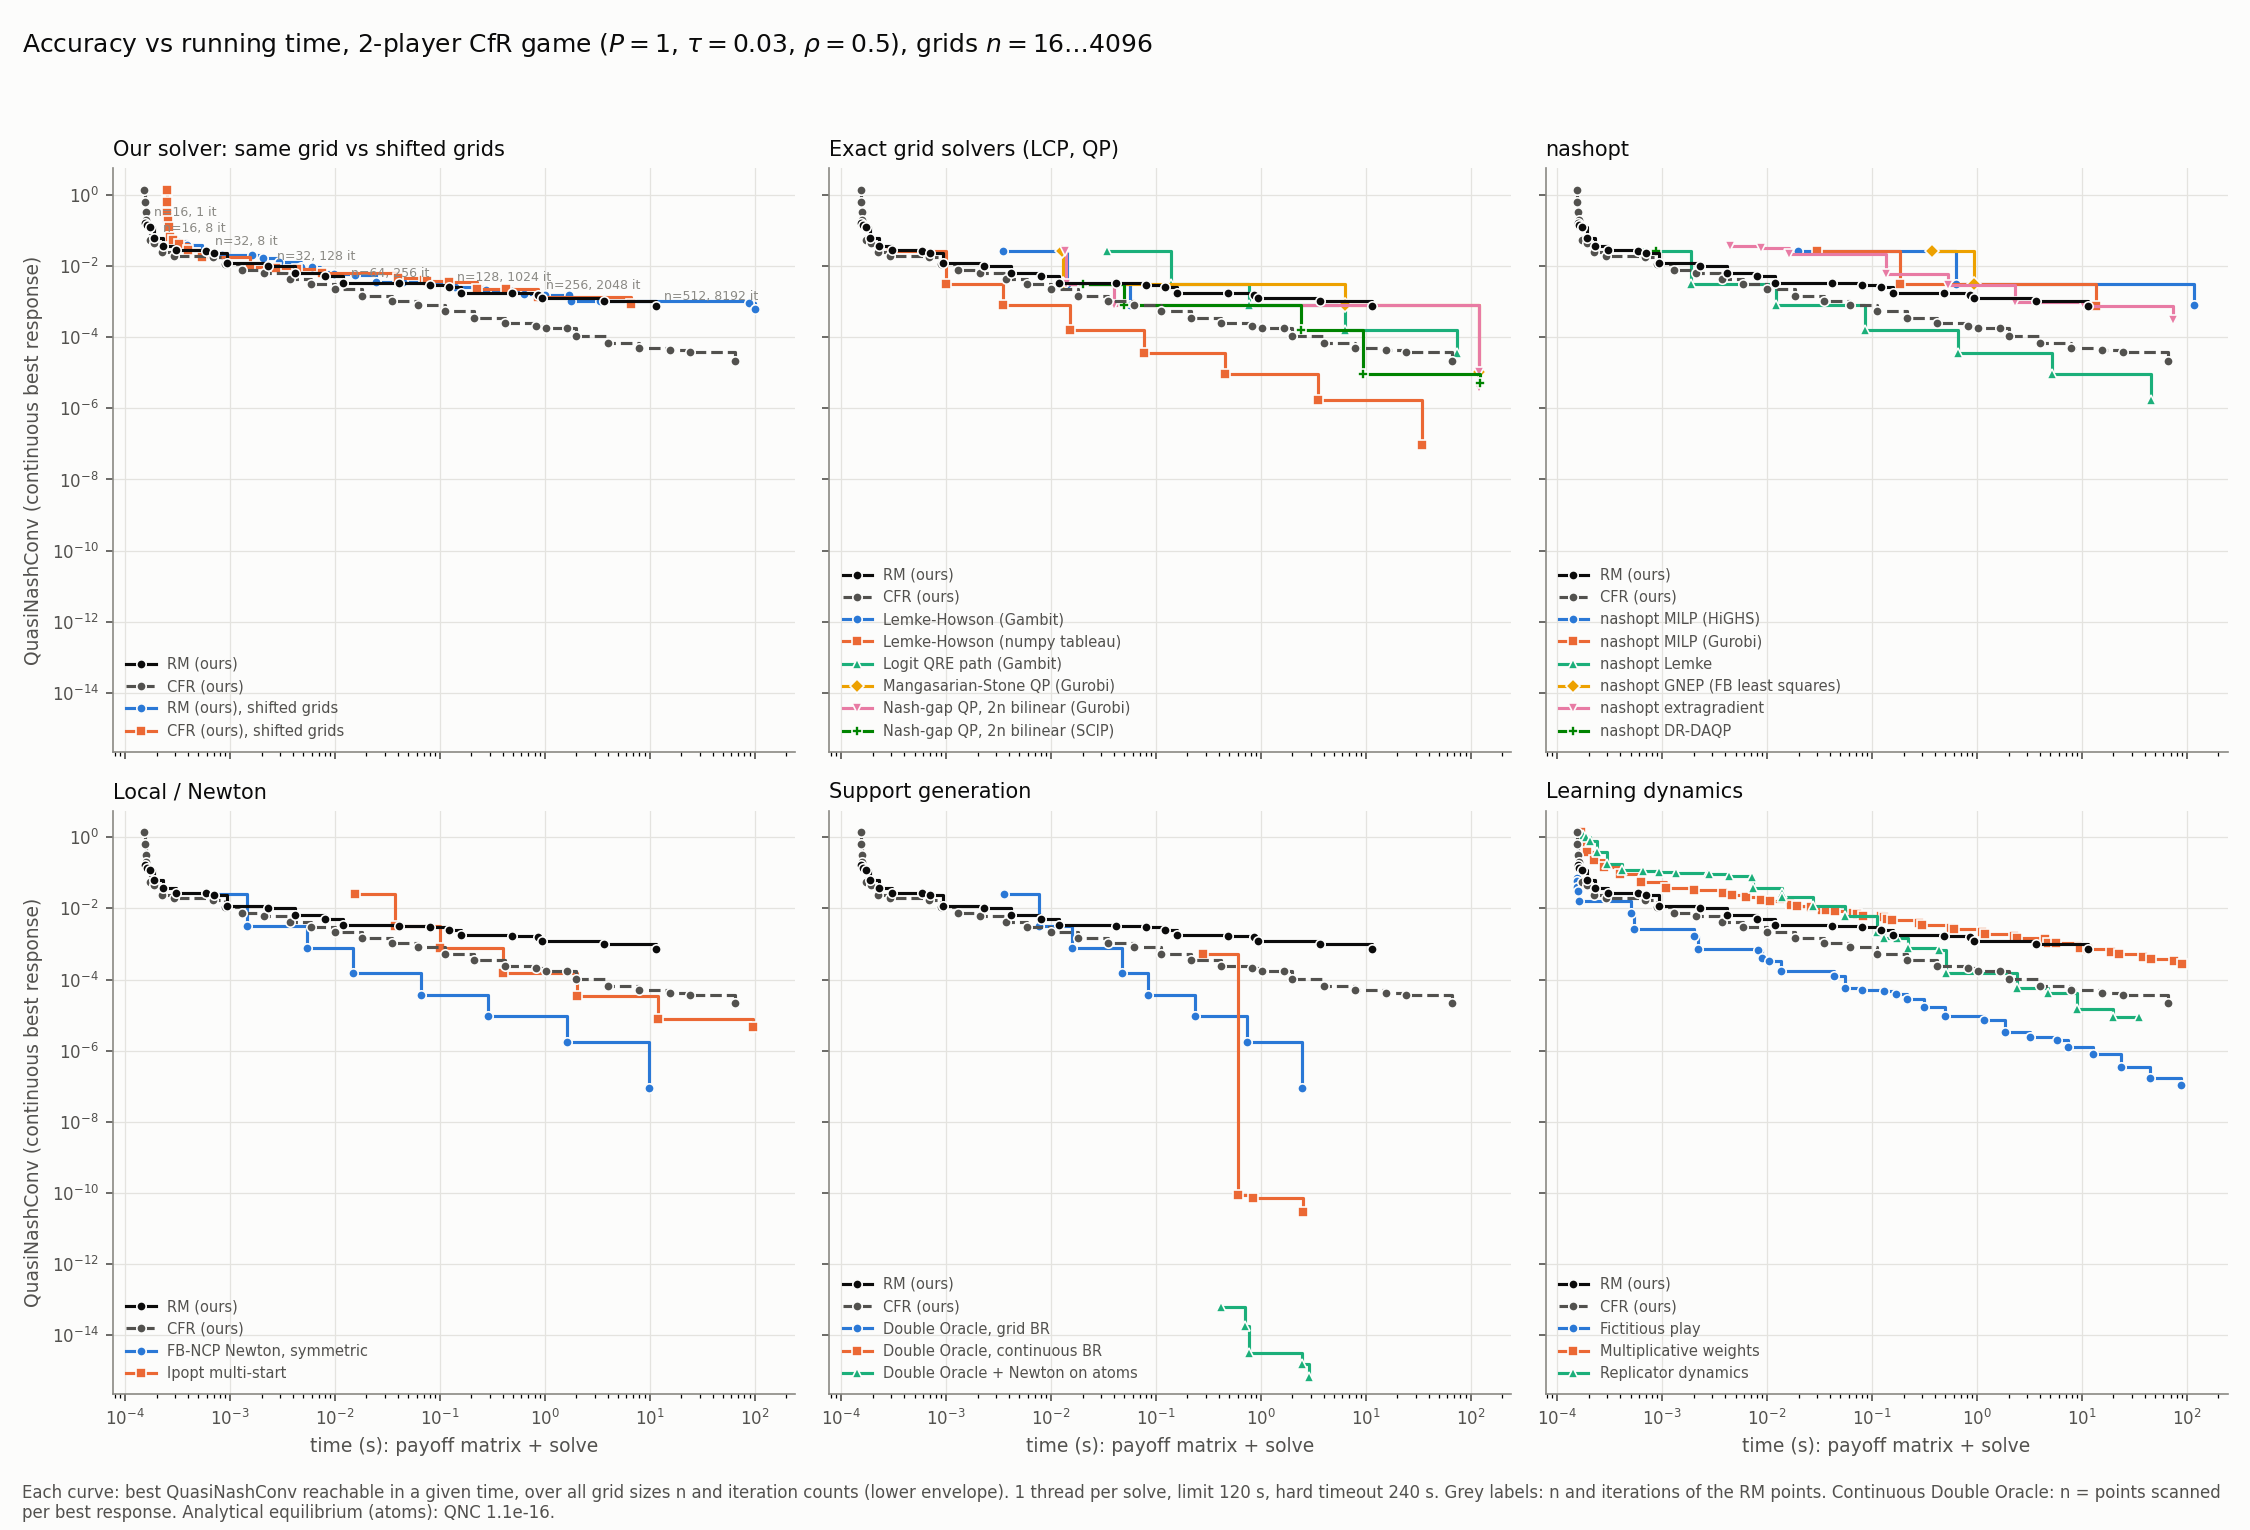
\includegraphics[width=\textwidth]{../../plots/benchmark_accuracy_time_tau=0.03.png}\\[2mm]
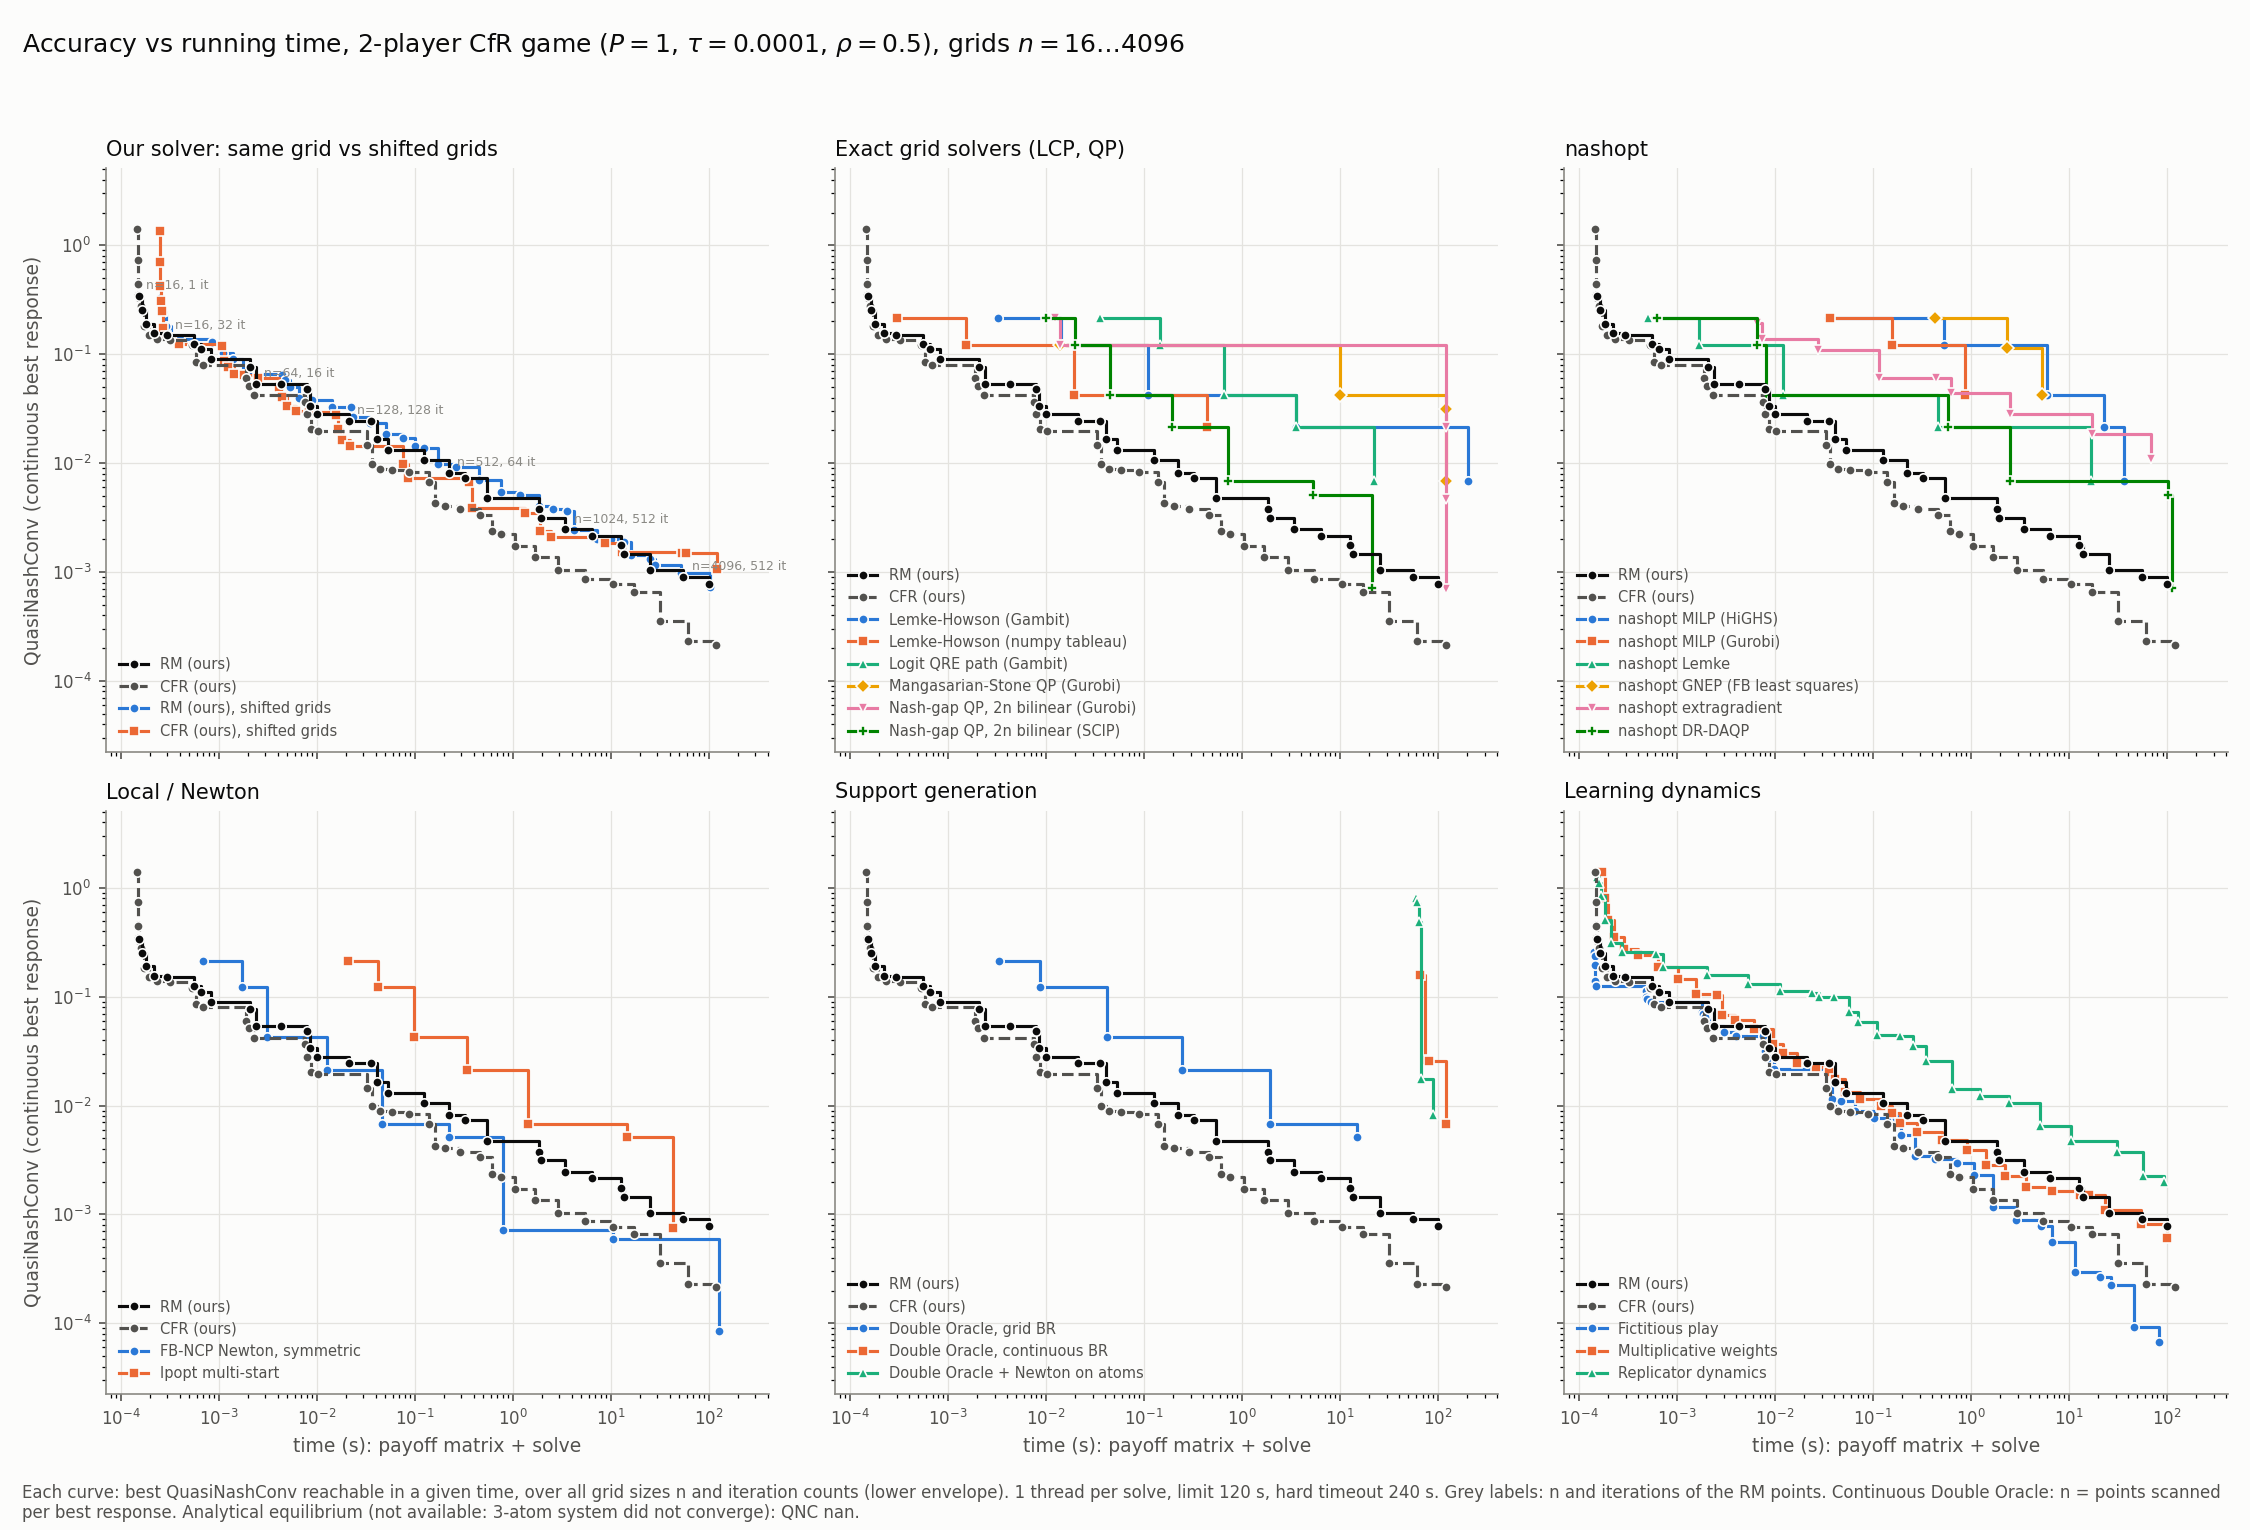
\includegraphics[width=\textwidth]{../../plots/benchmark_accuracy_time_tau=0.0001.png}
\caption{QNC against time, lower envelope over $(n,\text{iterations})$, for $\tau=0.03$ (top) and
$\tau=10^{-4}$ (bottom). The figure for $\tau=0$ is
\texttt{plots/benchmark\_accuracy\_time\_tau=0.svg}.}
\label{fig:tradeoff}
\end{figure}

\paragraph{Observations.}
For $\tau=0.03$, the continuous methods are far ahead: Double Oracle reaches $3\cdot10^{-11}$ and
Double Oracle + Newton the exact equilibrium, in about 3\,s. The grid methods cannot do better
than the exact equilibrium of the grid (QNC $9\cdot10^{-8}$ at $n=2048$); the fastest of them are
grid Double Oracle and FB-NCP Newton. CFR reaches $2\cdot10^{-5}$ and RM $7\cdot10^{-4}$.

For $\tau=10^{-4}$ and $\tau=0$ the equilibrium is, at the resolution of the grids, a density on
$[0, 0.387]$. Support generation then adds about one point per iteration and falls behind.
Fictitious play is the best method at $\tau=10^{-4}$ ($6.7\cdot10^{-5}$), FB-NCP Newton at
$\tau=0$ ($8.4\cdot10^{-4}$); CFR is 3 times worse at $\tau=10^{-4}$ and 1.5 times worse at
$\tau=0$. The Lemke--Howson paths become very
long on these nearly degenerate games (16\,000 pivots at $n=128$ for $\tau=0$, against 288 for
$\tau=0.03$): no Lemke--Howson implementation gives a better point than its result at $n=256$.

The two formulations of the Mangasarian--Stone program find a solution close to an equilibrium
within seconds for $n\le64$, but they cannot prove optimality (the lower bound stays negative)
and use the full time limit from $n=128$. The $2n$-bilinear version is better than the dense one.
The mixed-integer programs (nashopt) find no feasible point within 120\,s from $n=128$ with
Gurobi, and from $n=128$ or $n=512$ with HiGHS.

\section{Supports}

Table~\ref{tab:supexact} compares the Double Oracle solutions at $\tau=0.03$ with the exact
equilibrium. Double Oracle finds the 6 atoms but it never moves a point: when a best response lies
next to a true atom, the restricted equilibrium mixes two close points, whose weighted centre is
the atom. Most of the 16--70 points that it adds end with weight 0.

\begin{table}[H]
\centering\small
\begin{tabular}{lrcrrlcc}
\toprule
DO & $n$ & QNC & points added & weight $>0$ & points per atom & position error & weight error \\
\midrule
continuous & 64 & $3.8\cdot10^{-10}$ & 65 & 9 & 1,2,1,2,2,1 & $1.5\cdot10^{-5}$ & $3.8\cdot10^{-5}$ \\
continuous & 256 & $7.2\cdot10^{-11}$ & 61 & 9 & 1,1,2,1,2,2 & $3.1\cdot10^{-6}$ & $4.9\cdot10^{-6}$ \\
continuous & 1024 & $1.1\cdot10^{-10}$ & 68 & 11 & 1,2,2,2,2,2 & $7.3\cdot10^{-6}$ & $1.5\cdot10^{-5}$ \\
continuous & 4096 & $8.1\cdot10^{-11}$ & 70 & 9 & 1,2,1,2,2,1 & $1.4\cdot10^{-5}$ & $3.4\cdot10^{-5}$ \\
grid & 64 & $7.8\cdot10^{-4}$ & 16 & 9 & 1,2,1,1,2,2 & $2.5\cdot10^{-2}$ & $4.4\cdot10^{-2}$ \\
grid & 256 & $3.6\cdot10^{-5}$ & 26 & 10 & 1,1,2,2,2,2 & $3.8\cdot10^{-3}$ & $5.1\cdot10^{-3}$ \\
grid & 1024 & $1.7\cdot10^{-6}$ & 36 & 9 & 1,2,1,2,2,1 & $6.7\cdot10^{-4}$ & $1.2\cdot10^{-3}$ \\
grid & 4096 & $1.5\cdot10^{-7}$ & 45 & 9 & 1,1,2,1,2,2 & $2.1\cdot10^{-4}$ & $3.0\cdot10^{-4}$ \\
\bottomrule
\end{tabular}

\caption{Double Oracle against the exact 6 atoms, $\tau=0.03$. Each support point is assigned to
the nearest exact atom; errors are for the weighted centres and the summed weights.}
\label{tab:supexact}
\end{table}

\begin{table}[H]
\centering\small
\begin{tabular}{lrcrrc}
\toprule
Method & $n$ & QNC & weight $>10^{-9}$ & 99.9\% of the mass & range \\
\midrule
Fictitious play & 4096 & $6.7\cdot10^{-5}$ & 1584 & 1582 & $[0.000, 0.387]$ \\
CFR (ours) & 2048 & $2.1\cdot10^{-4}$ & 2048 & 791 & $[0.000, 0.386]$ \\
Double Oracle, grid BR & 512 & $5.1\cdot10^{-3}$ & 169 & 155 & $[0.000, 0.386]$ \\
Double Oracle, continuous BR & 512 & $6.7\cdot10^{-3}$ & 299 & 292 & $[0.000, 0.386]$ \\
\bottomrule
\end{tabular}

\caption{Supports at $\tau=10^{-4}$ (best result of each method).}
\label{tab:supsmall}
\end{table}

At $\tau=10^{-4}$ (Table~\ref{tab:supsmall}) fictitious play and CFR put their mass on the same
interval, which covers almost all grid points of $[0,0.387]$; fictitious play gives zero weight to
the other points, and CFR keeps a small weight on every point (the first, uniform iterations of the
average strategy).

\section{Double Oracle followed by Newton on the atoms}
\label{sec:hybrid}

\texttt{analytical.py} also grows a support, but it moves the atoms: for a support
$x_1<\dots<x_m$ it solves, in positions, weights and value $v$,
\[
\textstyle\sum_j u(x_i,x_j)w_j = v\ (\forall i),\qquad
\sum_j \partial_1 u(x_i,x_j)w_j = 0\ (x_i>0),\qquad \sum_j w_j=1 .
\]
The first-order condition places each interior atom at a local maximum of the deviation payoff;
Double Oracle has no such condition. The square system needs exactly the right number of atoms,
so we start from the Double Oracle solution and solve it with a Newton method that handles pairs:
two atoms closer than $\tau/10$ (the length scale of the payoff) merge into one, an atom whose
weight becomes non-positive leaves the support, the closest pair merges when the residual falls
by less than 10\% in 20 iterations, and the steps are damped (Levenberg--Marquardt). The Jacobian is
exact: $\partial_2 u$ follows from $u(a,b)+u(b,a)=1-\tilde r(a,b)-P(a+b)$. Among the start, the
states before each forced merge and the final state, we keep the one with the smallest continuous
best-response gap, measured on its own Sobol scan: on the scan of the Double Oracle oracle, the
start always looks converged.

\begin{table}[H]
\centering\small
\begin{tabular}{llcrcrrr}
\toprule
$\tau$ & start & QNC start & time (s) & QNC after & Newton (s) & atoms & merges \\
\midrule
$0.03$ & Double Oracle & $8.1\cdot10^{-11}$ & 8.7 & $3.2\cdot10^{-15}$ & 0.13 & 6 & 3+0 \\
$0.03$ & fictitious play & $8.5\cdot10^{-5}$ & 43 & $1.1\cdot10^{-14}$ & 0.16 & 6 & 7+0 \\
$0.01$ & Double Oracle & $8.9\cdot10^{-7}$ & 14 & $5.8\cdot10^{-9}$ & 26 & 32 & 12+31 \\
$0.01$ & fictitious play & $6.3\cdot10^{-5}$ & 43 & $2.6\cdot10^{-8}$ & 117 & 45 & 164+64 \\
$0.001$ & Double Oracle & $2.5\cdot10^{-6}$ & 305 & $6.0\cdot10^{-7}$ & 647 & 460 & 34+10 \\
$0.001$ & fictitious play & $2.1\cdot10^{-5}$ & 45 & $1.5\cdot10^{-5}$ & 646 & 765 & 14+4 \\
$0.0001$ & Double Oracle & $6.1\cdot10^{-1}$ & 303 & $6.1\cdot10^{-1}$ & 1.1 & 76 & 6+0 \\
$0.0001$ & fictitious play & $9.3\cdot10^{-5}$ & 51 & $9.3\cdot10^{-5}$ & 658 & 1584 & 0+1 \\
\bottomrule
\end{tabular}

\caption{Newton on the atoms after Double Oracle (300\,s) or fictitious play (60\,s), single
thread. Merges: collisions + forced merges.}
\label{tab:refine}
\end{table}

Table~\ref{tab:refine} gives the results. For $\tau=0.03$ both starts give the exact equilibrium
in 7 Newton steps. For $\tau=10^{-2}$ the error falls by a factor of about 150. For $\tau\le10^{-3}$
the support has hundreds of atoms, each Newton step costs seconds, and the gain is small or zero.
In the benchmark (Table~\ref{tab:all}) the method uses half of the time limit for Double Oracle
and half for Newton; it does not apply to $\tau=0$ (the payoff is not smooth).

\section{More than two players}

\paragraph{Game.} With $n$ players and independent failures ($\rho=0$), among the players that do
not fail, player $i$ wins $R$ with probability $e^{r_i/\tau}/\sum_{j} e^{r_j/\tau}$; for $n=2$
this is the friction model above. If the $n-1$ opponents play the mixed strategy $(a_k,w_k)$,
the identity $1/x=\int_0^\infty e^{-tx}dt$ with $t=e^s$ gives
\[
U(r) = -Pr + (1-r)\int e^{s-e^{s}}\,G(s,r)^{n-1}\,ds,\qquad
G(s,r)=\sum_k w_k\big[a_k+(1-a_k)\exp(-e^{s+(a_k-r)/\tau})\big],
\]
one integral whatever $n$. This formula agrees with \texttt{game.py} for $n=2$ to $3\cdot10^{-14}$
and with a Monte Carlo simulation for $n=3,4$.

\paragraph{Multiple Oracle.} We apply Algorithm 1 of Kroupa and Votroubek \cite{kroupa2021}. The
game is symmetric, so the players share one strategy set and one best response; the restricted
game is the symmetric complementarity problem in the weights, solved by Fischer--Burmeister
Newton followed by Newton on the support. Its payoffs are polynomials of degree $n-1$ in the
weights, so each restricted solve is a nonlinear problem, but it has $k$ unknowns and not a
payoff table of $k^n$ entries.

\begin{table}[H]
\centering\small
\begin{tabular}{p{3cm}p{6.3cm}p{6.3cm}}
\toprule
 & Double Oracle \cite{mcmahan2003} & Multiple Oracle \cite{kroupa2021} \\
\midrule
Games & two players, zero-sum, finite & $n$ players, general-sum, compact action sets, continuous payoffs \\
Restricted game & linear program & $n$-player Nash equilibrium (PATH in \cite{kroupa2021}; here a symmetric complementarity problem) \\
Best response & over a finite set & global optimization over the continuous set \\
Stop & finite: the action sets are finite & finite for $\varepsilon>0$; for $\varepsilon=0$ every limit point is an equilibrium \\
\bottomrule
\end{tabular}
\caption{Standard Double Oracle and Multiple Oracle.}
\end{table}

\begin{table}[H]
\centering\small
\begin{tabular}{rccrrrrrc}
\toprule
$n$ & NashConv & check & time (s) & iterations & $|X|$ & weight $>0$ & atoms & mass at 0 \\
\midrule
2 & $2.9\cdot10^{-7}$ & $2.9\cdot10^{-7}$ & 417 & 56 & 56 & 12 & 6 & 0.106 \\
3 & $1.4\cdot10^{-7}$ & $1.4\cdot10^{-7}$ & 420 & 66 & 66 & 18 & 9 & 0.165 \\
5 & $2.2\cdot10^{-9}$ & $1.9\cdot10^{-7}$ & 404 & 71 & 71 & 13 & 8 & 0.415 \\
10 & $8.5\cdot10^{-11}$ & $1.2\cdot10^{-10}$ & 293 & 66 & 66 & 11 & 7 & 0.720 \\
\bottomrule
\end{tabular}

\caption{Multiple Oracle, $\tau=0.03$, $P=1$, $\rho=0$, 400\,s limit, 2 threads. Check: NashConv with a finer
best response. Atoms: groups of support points less than $2\cdot10^{-3}$ apart.}
\label{tab:multi}
\end{table}

Table~\ref{tab:multi} gives the results. The number of atoms stays small (6 to 9) and the mass
at zero risk grows with $n$. For $n=5$ the oracle reports $2.2\cdot10^{-9}$ but the finer check
gives $1.9\cdot10^{-7}$: the oracle scan ($2^{12}$ points) misses the best deviation. Removing the
zero-weight strategies after each restricted solve (not in \cite{kroupa2021}) makes the algorithm
cycle: for $n=2$, after 100 iterations the set still has 2 strategies and NashConv repeats the
sequence $0.56, 0.43, 0.32, 0.24, 0.20$. The restricted solves are much slower than in the
two-player case, where the restricted game is bilinear and its support system linear: on the same
game ($n=2$, $\rho=0$), the two-player Double Oracle reaches $1.6\cdot10^{-10}$ in 1.7\,s,
against $2.9\cdot10^{-7}$ in 417\,s for the Multiple Oracle (\texttt{bench/multiplayer/checks.json}).

\section{Limits}

All two-player results are for $P=1$ and $\rho=0.5$, and the $n$-player results for $\tau=0.03$ and
$\rho=0$. The time limit (120\,s) favours methods that give a usable point early. Gurobi used a
full license (WLS); an earlier size-limited license stopped the Gurobi methods at 2000 variables.

\begin{thebibliography}{99}\small
\bibitem{abraham2023} L. Abraham. A game of Competition for Risk. arXiv:2305.18941, 2023.
\bibitem{mangasarian1964} O.L. Mangasarian and H. Stone. Two-person nonzero-sum games and quadratic programming. \emph{Journal of Mathematical Analysis and Applications}, 9:348--355, 1964. \url{https://doi.org/10.1016/0022-247X(64)90021-6}
\bibitem{lemke1964} C.E. Lemke and J.T. Howson. Equilibrium points of bimatrix games. \emph{Journal of the SIAM}, 12(2):413--423, 1964.
\bibitem{mcmahan2003} H.B. McMahan, G.J. Gordon and A. Blum. Planning in the presence of cost functions controlled by an adversary. \emph{ICML}, 2003.
\bibitem{kroupa2021} T. Kroupa and T. Votroubek. Multiple oracle algorithm to solve continuous games. arXiv:2109.04178.
\bibitem{hart2000} S. Hart and A. Mas-Colell. A simple adaptive procedure leading to correlated equilibrium. \emph{Econometrica}, 68(5):1127--1150, 2000.
\bibitem{zinkevich2007} M. Zinkevich, M. Johanson, M. Bowling and C. Piccione. Regret minimization in games with incomplete information. \emph{NIPS}, 2007.
\bibitem{brown1951} G.W. Brown. Iterative solution of games by fictitious play. In \emph{Activity Analysis of Production and Allocation}, 1951.
\bibitem{robinson1951} J. Robinson. An iterative method of solving a game. \emph{Annals of Mathematics}, 54:296--301, 1951.
\bibitem{freund1999} Y. Freund and R.E. Schapire. Adaptive game playing using multiplicative weights. \emph{Games and Economic Behavior}, 29:79--103, 1999.
\bibitem{taylor1978} P.D. Taylor and L.B. Jonker. Evolutionarily stable strategies and game dynamics. \emph{Mathematical Biosciences}, 40:145--156, 1978.
\bibitem{mckelvey1995} R.D. McKelvey and T.R. Palfrey. Quantal response equilibria for normal form games. \emph{Games and Economic Behavior}, 10:6--38, 1995.
\bibitem{turocy2005} T.L. Turocy. A dynamic homotopy interpretation of the logistic quantal response equilibrium correspondence. \emph{Games and Economic Behavior}, 51:243--263, 2005.
\bibitem{fischer1992} A. Fischer. A special Newton-type optimization method. \emph{Optimization}, 24:269--284, 1992.
\bibitem{ipopt} A. W\"achter and L.T. Biegler. On the implementation of an interior-point filter line-search algorithm for large-scale nonlinear programming. \emph{Mathematical Programming}, 106:25--57, 2006.
\bibitem{sandholm2005} T. Sandholm, A. Gilpin and V. Conitzer. Mixed-integer programming methods for finding Nash equilibria. \emph{AAAI}, 2005.
\bibitem{korpelevich1976} G.M. Korpelevich. The extragradient method for finding saddle points and other problems. \emph{Ekonomika i Matematicheskie Metody}, 12:747--756, 1976.
\bibitem{nashopt} A. Bemporad. NashOpt: a Python library for computing generalized Nash equilibria. arXiv:2512.23636.
\bibitem{gambit} R. Savani and T.L. Turocy. Gambit: the package for computation in game theory, version 16.7. \url{https://www.gambit-project.org}
\bibitem{mathecon} Math-econ-code. Nash equilibria of bimatrix games. \url{https://math-econ-code.github.io/gt_nash.html}
\end{thebibliography}

\end{document}
